\chapter[Experimental setup]{Experimental setup}

At CERN the high-gradient test are carried on the three X-band test stands (XBOXs), that are setups able to provide the necessary high power RF pulses to the structure under tests. Nevertheless for the tests described in this work the presence of the beam inside the accelerating cavity is necessary, and is provided by the electron linac of the CTF3. 


\section[Linac and dogleg]{The LINAC and the Dogleg}

\subsection[The test setup]{The test setup}
As mentioned in the first chapter, the main goal of the CTF3 is to demonstrate the feasibility of the CLIC acceleration scheme. For this reason, the linac is realised using the conventional $3\,GHz$ technology, that after the recombination process will lead to the beam frequency of $12\,GHz$. 

Given that the tests of high-gradient cavities is not the design goal of the facility, in the following sections only the relevant part of the setup for the brakdown experiments will be described. The full description of the CTF3 accelerator complex is widely described elsewhere \cite{CLIC:cdr,CTF:drive_beam,ctf3:dr}.

To realise high-gradient structure tests, a beam line parallel to the linac have been set up. The two beam lines are connected by an oblique segment, giving the characteristic shape that is the origin of the name \textit{Dogleg}.

The parameters of the beam that is possible to produce are reported in the table \ref{beam_par_dogleg}


\begin{table}
  \centering
    \begin{tabular}{ c l }
    \hline
    Current 		&	up to $1.6\,A$\\
    Pulse length		&	up to $250\,ns$\\
    Energy			&	up to $130\, MeV$\\
    Reptition freq.	&	$0.83\,-\,50\, Hz$\\

    \hline
    \end{tabular}
\caption{Beam parameters achievable in the Dogleg \cite{NavarroQuirante:2025954}}
\label{beam_par_dogleg}
\end{table}



\subsubsection{Injector}

The production of the beam is realised by a 140-kV thermoionic gun, designed to deliver $5\,A$ of current in nominal operation conditions.
The gun is followed by a S-band prebuncher and a 17 cell travelling-wave buncher. These structures are followed by two 1-m long accelerating structures. The beam dimension in this initial phase is controlled using solenoids, that continue up to the second accelerating structure \cite{ctf:injector}.

Downstream the injector a magnetic chicane with collimators is installed to eliminate off-energy particles and to perform the bunch compression  \cite{Braun:999488}.

\subsubsection{Linac}

In the linac are installed three modules composed of two S-band accelerating structures operating at $3\,GHz$. The accelerating structures consist of 32 regular cells, operating in the $2\pi/3$ mode. The daping of HOMs is guaranteed by the radial slots in the iris containing SiC loads.

The focusing is realised by triplets of quadrupoles, coupled with dipole correctors. The beam energy can be measured in the spectrometers in sector 4 and 10.



\subsubsection{The dogleg}

 The layout of the dogleg is exploited in figure \ref{dolaut}.




\begin{landscape}
\begin{center}

\begin{figure}[h]
\centering 
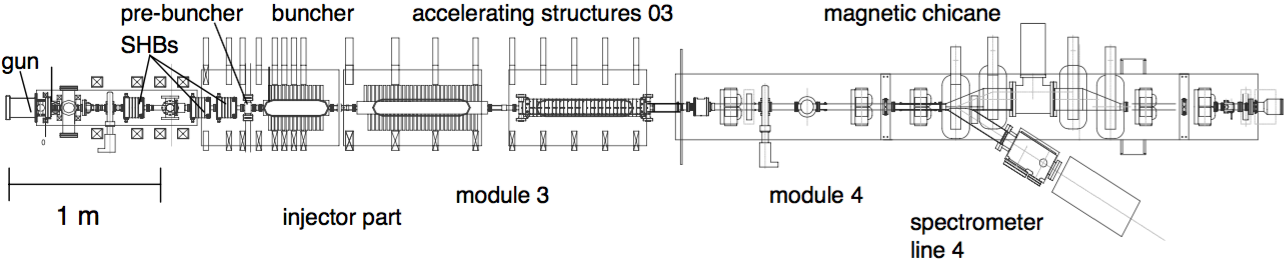
\includegraphics[width=23cm,keepaspectratio]{pictures/Injector}
\caption{Layout of the injector and the magnetic chicane}
\label{injlayout}
\end{figure}

\vspace{20mm}

\begin{figure}[h]
\centering 
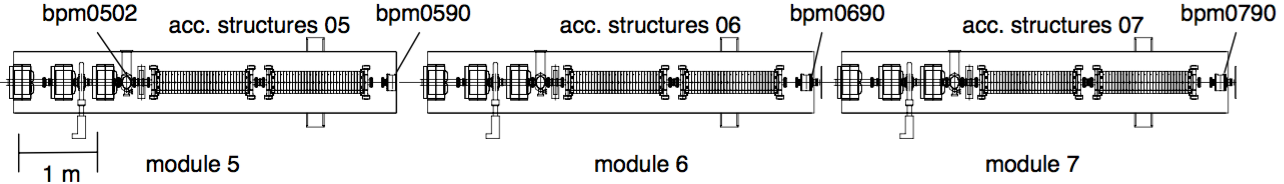
\includegraphics[width=23cm,keepaspectratio]{pictures/girder5-7}
\caption{Layout of the linac up to module 7}
\label{injlayout}
\end{figure}

\end{center}
\end{landscape}



\begin{landscape}
\begin{figure}
\centering 
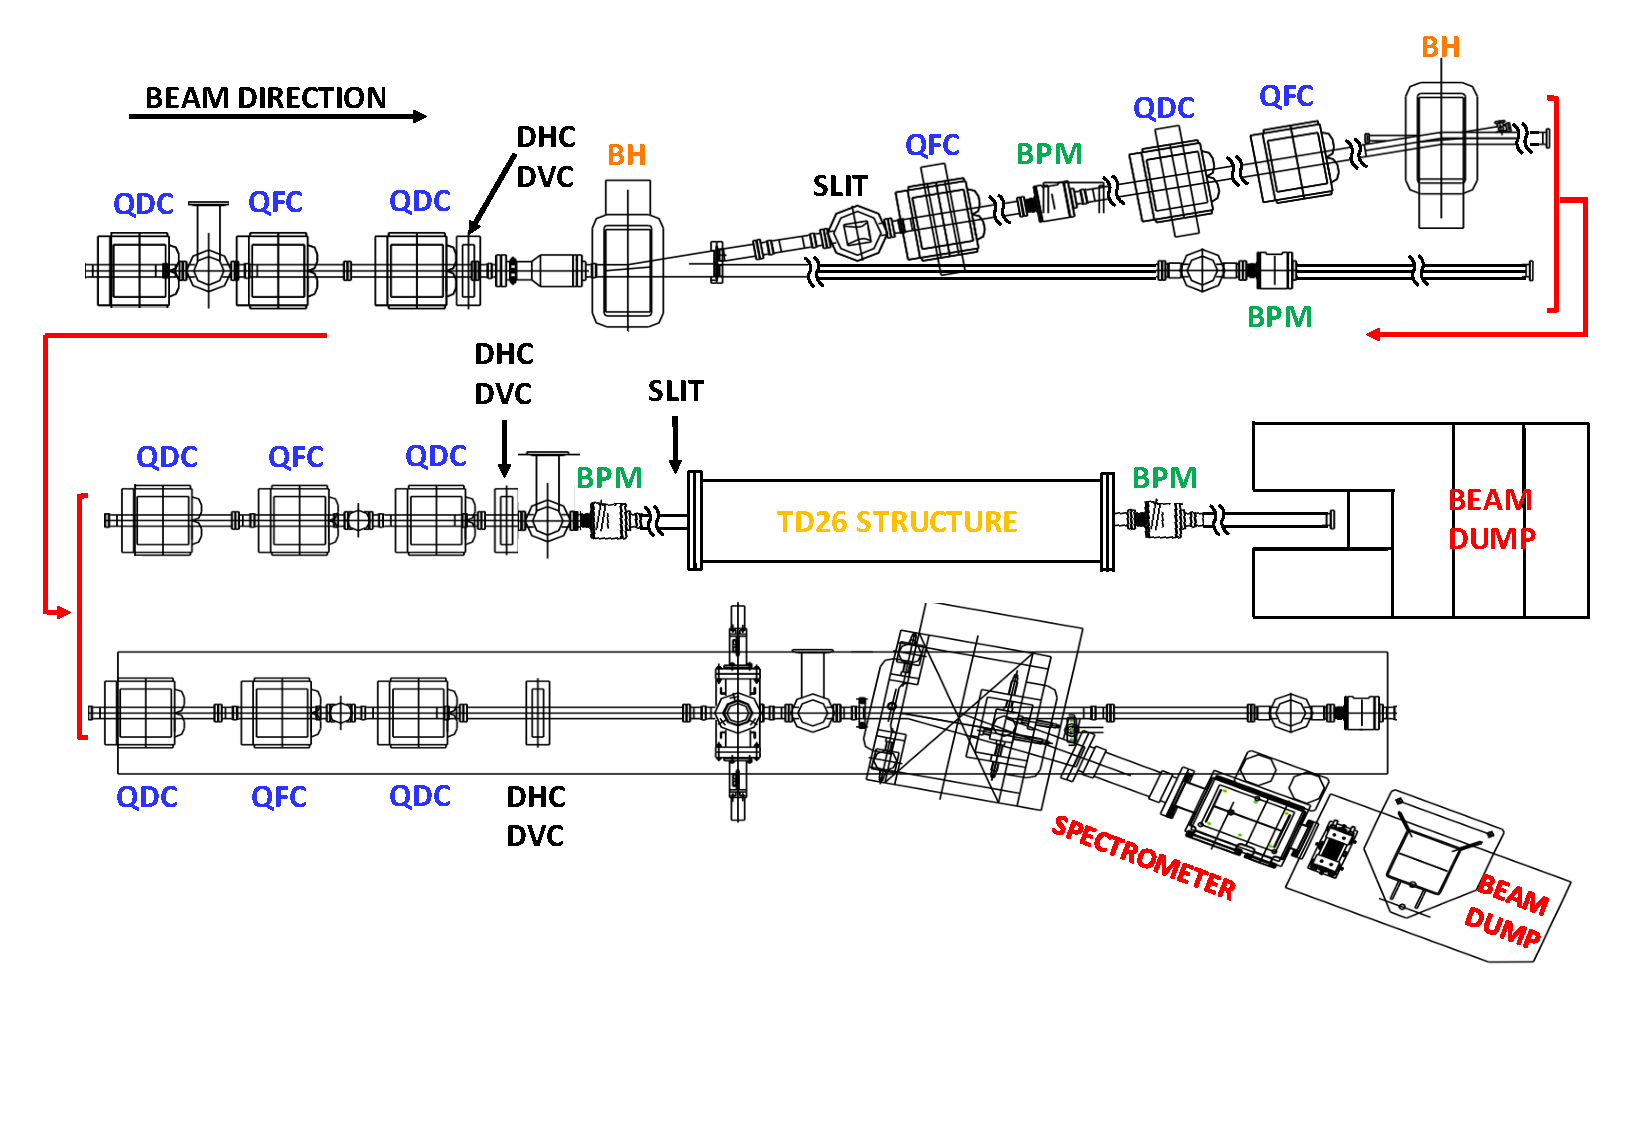
\includegraphics[scale=0.78]{pictures/modified_pets.pdf}
\caption{Simplified layout of optics and beam instrumentation of the dogleg line, adapted from technical drawings and facility layout \cite{EDMS:CTF3}. The beam for this section come from the end of the module 7. Legenda: QFC(QDC): focusing(defocusing) quadrupole; DHC(DVC): horizontal(vertical) dipole corrector; BH: bending magnet in horizontal plane; BPM: beam position monitor}
\label{dolaut}
\end{figure}
\end{landscape}


\subsubsection{RF power source}




\subsection[Comparison of setup and CLIC design]{Comparison of setup and CLIC design}



\section[RF power generation]{RF power generation}



\section[DAQ system]{DAQ system}

\subsection[Hardware]{Hardware}

\subsection[Online triggers]{Online triggers}

describe the online, but then the offline is in the next chapter

\section[Other systems]{Other systems}

mention here thermal systems for the structure and something else ???

